Die Testdaten zum F�llen der Tabellen werden mit einem Datengenerator erzeugt.

\section{Analyse}
Der Datengenerator soll die Testdaten f�r die vier Tabellen 
\begin{itemize}
	\item Kunde,
	\item Produkt,
	\item Warenkorb,
	\item WarenkorbProdukt
\end{itemize}
erzeugen und in die Tabellen schreiben. Dabei sollen dem Generator vier Parameter beim Start �bergeben werden:
\begin{enumerate}
	\item die Anzahl der zu erzeugenden Kunden
	\item die Anzahl der zu erzeugenden Produkte
	\item die Anzahl der Warenk�rbe pro Kunde
	\item die Anzahl der Produkte im Warenkorb
\end{enumerate}

Der Generator muss f�r alle beliebigen Startparameter die Tupel der einzelnen Tabellen korrekt miteinander verkn�pfen. Deswegen erzeugt der Generator auch die Prim�r- und Fremdschl�ssel der Tupel selbst. 
Die maximale Anzahl der Warenk�rbe ergibt sich aus der Anzahl der Kunden * der Anzahl der Warenk�rbe pro Kunde. In der Warenkorbtabelle m�ssen bei einer Anzahl von z.B. 10 Warenk�rben pro Kunde auch je 10 Warenk�rbe existieren, die mit ihrem Fremdschl�ssel auf den jeweiligen Kunden zeigen. In der Warenkorbtabelle sollen im Datum alle Monate des Jahres 2011 gleichm��ig verteilt vorkommen. 

Die maximale Anzahl der Bestellzeilen ergibt sich aus der Anzahl der Kunden * der Anzahl der Warenk�rbe pro Kunde * der Anzahl der Produkte in einem Warenkorb. Die m�glichen Produkte sollen gleichm��ig �ber alle Bestellzeilen verteilt sein. In der WarenkorbProdukt-Tabelle m�ssen bei einer Anzahl von z.B. 7 Produkten im Warenkorb auch je 7 Bestellzeilen existieren, die mit ihrem Fremdschl�ssel auf den jeweiligen Warenkorb zeigen.

F�r jede Tabelle soll ausgegeben werden, wieviel Zeit der Generator insgesamt f�r den Schreibvorgang ben�tigte. Damit wird es auch m�glich, die Schreibperformance einer Datenbankkonfiguration zu messen und auszuwerten.

\subsection{Anwendungsfalldiagramm}

Die Abbildung \ref{fig:AnwendungsfalldiagrammDatengenerator} auf Seite \pageref{fig:AnwendungsfalldiagrammDatengenerator} zeigt das Anwendungsfalldiagramm des Prototypen.

\subsection{User Stories}

1. AF - Datengenerator mit Aufrufparametern ausf�hren
Um die Testdaten zu generieren und in die Tabellen zu schreiben ruft der Anwender den Datengenerator als Jar-Datei �ber die Kommandozeile auf und �bergibt ihm die folgenden vier Aufrufparameter in gegebeneer Reihenfolge:
\begin{enumerate}
	\item die Anzahl der zu erzeugenden Kunden
	\item die Anzahl der zu erzeugenden Produkte
	\item die Anzahl der Warenk�rbe pro Kunde
	\item die Anzahl der Produkte im Warenkorb
\end{enumerate}

2. AF - Zeiten f�r die Schreibvorg�nge �bernehmen
Der Anwender notiert sich die vom Generator auf der Konsole ausgegebenen Gesamtzeiten der einzelnen Schreibvorg�nge.

3. AF - Anzahl der insgesamt geschriebenen Tupel pro Tabelle �bernehmen
Der Anwender notiert sich die auf der Konsole ausgegebenen Werte der vom Generator insgesamt geschriebenen Tupel f�r jede Tabelle.

\subsection{Nichtfunktionale Anforderungen}
Da im sp�teren Projektverlauf leicht neue Tabellen hinzukommen k�nnen, soll die Anwendung leicht anpassbar sein.

\subsection{Analyseklassendiagramm}
Die Abbildung \ref{fig:AnalyseDatengenerator} auf Seite \pageref{fig:AnalyseDatengenerator} zeigt das Analyseklassendiagramm des Datengenerators.

\subsection{UI-Mockup}
Die Abbildung \ref{fig:UI-MockUp} auf Seite \pageref{fig:UI-MockUp} zeigt das UI-Mockup des Datengenerators.



\begin{figure}[htp]
\centering
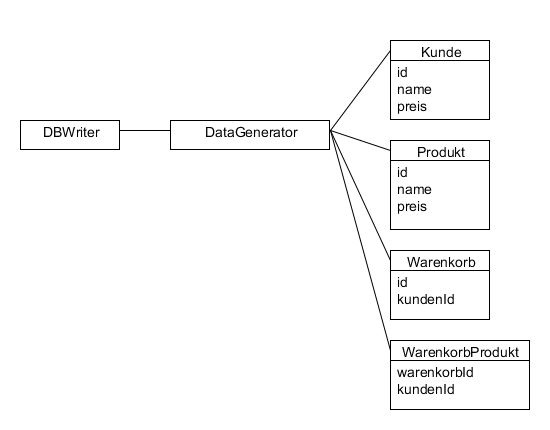
\includegraphics[width=0.8\textwidth]{Ingo/Bilder/AnalyseDatengenerator.png}
\caption{Analyse Datengenerator}
\label{fig:AnalyseDatengenerator}
\end{figure}

\begin{figure}[htp]
\centering
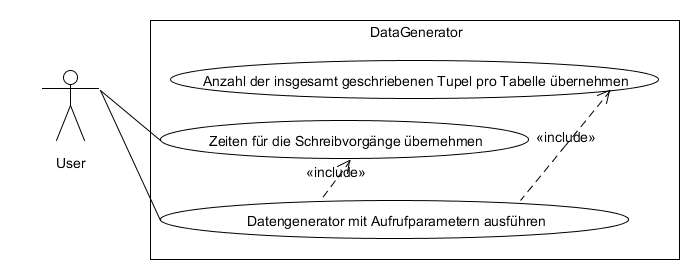
\includegraphics[width=0.8\textwidth]{Ingo/Bilder/AnwendungsfalldiagrammDatengenerator.png}
\caption{Anwendungsfalldiagramm Datengenerator}
\label{fig:AnwendungsfalldiagrammDatengenerator}
\end{figure}


\begin{figure}[htp]
\centering
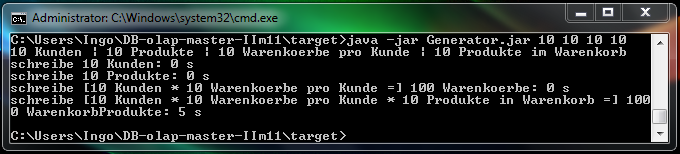
\includegraphics[width=0.8\textwidth]{Ingo/Bilder/UIMockUp.png}
\caption{UI-MockUp}
\label{fig:UI-MockUp}
\end{figure}